\chapter{Escalamiento}

Scrum es aconsejable para ser óptimo en equipos chicos y proyectos pequeños, con agrupación de personas de múltiples disciplinas en un solo equipo para maximizar el ancho de banda de las comunicaciones, la visibilidad y la confianza. Esto sucede porque cuando los equipos son grandes aumenta el acoplamiento de individuaos complejizando las comunicaciones y dificultando la coordinación y el buen desarrollo de las reuniones Scrum. Además se desprende del principio o Ley de Brooks , que cuando se agregan personas a un proyecto o equipo aumentan los canales de comunicación pudiendo generar sobrecarga de comunicación. Por este motivo y desde un punto de vista purista, cuando se quiere implementar Scrum en proyectos grandes que requieren muchas personas, en su forma ortodoxa, no es recomendable. Pero se han encontrado maneras organizativas para aplicar Scrum en estos casos. Una forma es el uso de equipos Scrum de características, equipos Scrum de componentes y el uso de "Scrum de Scrum".

\section{Equipos de características}

Abordar el problema de proyectos grandes con "Equipos Scrum de características" consiste en la conformación de equipos totalmente multi-funcionales, capases de operar en todos los niveles de la arquitectura del producto con el fin de ofrecer las características centradas en el cliente. O sea que cada equipos trabaja sobre determinadas características de producto (Features) o PBIs desarrollando todos los niveles del sistema a desarrollar. En este sentidos, los equipos son homogéneos entre si pero eterogéneos internamente, con integrantes de habilidades diversas y características profesionales multidisciplinares. Para lograr esto se debe conformar una organización de aprendizaje donde los equipos practican el aprendizaje continuo, donde aprenden para abarcar los componentes arquitectónicos. 

\begin{figure}[h]
  \centering
  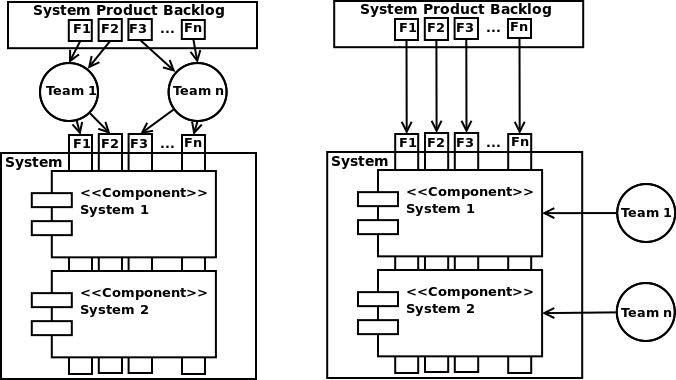
\includegraphics[width=0.99\textwidth]{ScrumTeamsByFeaturesAndByComponents}
  \caption{Equipos de Características y Equipos de Componentes.}
  Equipos de Características (izquierda) y Equipos de Componentes (derecha)
  \centering
  \label{fig:ScrumTeamsByFeaturesAndByComponents} %\ref{fig:ScrumTeamsByFeaturesAndByComponents}
\end{figure}

En esta arquitectura de organización es necesario coordinar el trabajo de los diferentes equipos. Los Scrum Master deben reunirse con regularidad, promoviendo la transformación a travez de una lista visible de los impedimentos de organización. Los Scrum Master, además deberan estar familiarizados con biografía relacionada a este proble de escalabilidad como "Scaling Lean and Agile Development" \cite{Larman-Vodde-2008}.

\section{Equipos de componentes}

Abordar el problema de proyectos grandes con "Equipos Scrum de componentes" (ver figura \ref{fig:ScrumTeamsByFeaturesAndByComponents}) consiste en que cada equipo sólo es responsable de la ejecución de ciertos componentes dedicados en el sistema de los cuales el equipo es dueño de su desarrollo. Desde esta perspectiva se pueden tener equipos dedicados por capas (capa front-end, capa de servicios, capa de persistencia) y por componentes de arquitectura de software (diferentes componentes como librerías, servicios o subsistemas).

Para terminar una PBI o historia de usuario hay en la mayoría de los casos la necesidad de dividir las historias en partes más pequeñas que podrían ser implementadas dentro de un solo componente. Además se genera dependencias entre los diferentes equipos haciendo necesario procesos de integración periódica y coordinación de equipos. En muchos casos, una sola historia de usuario no se puede implementar dentro de un único sprint y, en su defecto, depende de los resultados de otras historias desarrolladas por otro equipo que aún no están disponibles. A esto se lo llama "pipeline" y debe evitarse en lo posible o gestionarse apropiadamente.

La ventaja de utilizar equipos de componentes es que es más fácil asegurar una determinada arquitectura del sistema. Por ejemplo si se quiere asegurar una Arquitectura SOA o una de Microservicios que está orientada a componentes. Esta idea está, entre otras cosas, basada en la "Ley de Conway"\footnote{Conway's Law \cite{Conway-1968} no es exactamente una ley, sino que es más bien una observación que Conway publicó en 1968.} que sugiere que las organizaciones pueden replicar su arquitectura en los productos que ellas producen \cite{Martin-Fowler-2014}. 

Por otro lado, puede tener como desventaja que las personas se pueden especializar sólo en pequeñas partes del sistema y el conocimiento global sobre el sistema en su conjunto podría perderse \cite{Scrum-Institute-2015}. En este caso podría tener lugar una optimización local, ya que el equipo a veces puede tomar decisiones que están optimizados para el componente individual, pero las mejores soluciones desde una perspectiva del sistema total podrían haber sido desestimadas u oviadas.

\section{Scrum de Scrum}

Scrum de Scrum es una forma de organización y técnica para escalar Scrum a grupos grandes de personas. Consiste en distinguir un integrante con el rol de Embajador, denominado "Ambassador", por cada Equipo Scrum \cite{Stefanini-2013}. El Embajador será quien participará en reuniones Daily con Embajadores de otros equipos. A esta reunión de Embajadores se la llama "Scrum de Scrum". Habitualmente se usa que el rol de Embajador lo desempeñe el Scrum Master, pero puede ser desempeñado por otro integrante del Equipo de Desarrollo. La reunión “Scrum de Scrum” se comporta como una Daily donde los Embajadores reportan la cituación de su equipo y sus impedimentos.


